\documentclass[10pt,twocolumn]{article} 
\usepackage{simpleConference}
\usepackage{times}
\usepackage{graphicx}
\usepackage{amssymb}
\usepackage{url,hyperref}
\usepackage{enumitem}
\usepackage{float}
\usepackage{amsmath}
\usepackage{subcaption}

\usepackage{booktabs,siunitx}

% Settings %
\graphicspath{{./figures/}}
\sisetup{table-format=2.1}

\begin{document}

\title{Artificially Generating Percussive Tracks \\ \large{6.882 Final Project}}

\author{Juan M Ortiz \\
\today
\\
\\
juanmoo@mit.edu  \\
}

\maketitle

\section{Introduction}
  The idea of utilizing artificial intelligence to create music is by no means a novel topic. Some of the first recorded attempts to generate music algorithmically date all the way back to the 1960s (Zaripov, 1960) \cite{zaripov1960algorithmic} with computers that were still utilizing vacuum tubes and is still a topic of research in labs like Google Magenta and OpenAI today. In this paper, we explore two different approaches to generate drum tracks and analyse their capabilities and limitations. The first will be a simple approach that treats track generation as a time-series forecast problem using an LSTM network architecture. We observe that this approach fails to capture long term structure and is thus ineffective at generating longer sequences. The second approach follows some of the experiments in (Roberts et al., 2018) \cite{roberts2018hierarchical} and attempts to mitigate this problem using a recurrent Variational Autoencoder (VAE) with a \textit{hierarchical} decoder. Rather than directly decoding the latent code produced by the VAE back into a sequence, the latent code is us used to generate several embeddings which are then independently decoded and concatenated to create the final piece. This architecture encourages each subsequence to utilize the latent code and we observe does better empirically at reconstructing and generating longer sequences.
  m 

\section{Background}
The following sections provide a brief exposition to the ideas utilized in the experiment section. 

\subsection{Time-Series Forecasting}
A common way to tackle music generation is to treat it as a time-series forecast problem. Formally, a time-series is a sequence of successive data points that are indexed by time with constant spacing. A time-series forecasting problem then refers to utilizing a model to predict future values based on previous observations. In our case, the data points will correspond to the encoded representations of the combination of instruments being used at different points in time and each time-step will correspond to a 16th note interval. 

With this framework, if we let $x_t$ correspond to the encoding of instruments played at time $t$, we can summarize our simple approach described in \textbf{3.1} as a time-series forecasting problem that predicts $x_{t}$ from the samples $x_{t - j}$ such that $j \in [1, t]$.

\subsection{Variational Autoencoders}

At a fundamental level, an autoencoder is a type of network that attempts to learn an efficient data representation in an unsupervised manner. A common constraint utilized to encourage learning this representation is to force the data in question to pass through a lower-dimensional latent space before attempting to be reconstructed on the output side of the network. Ideally, this forces the latent code to capture important features about the input data while ignoring irrelevant information and/or noise.

\begin{figure}[H]
  \center{
    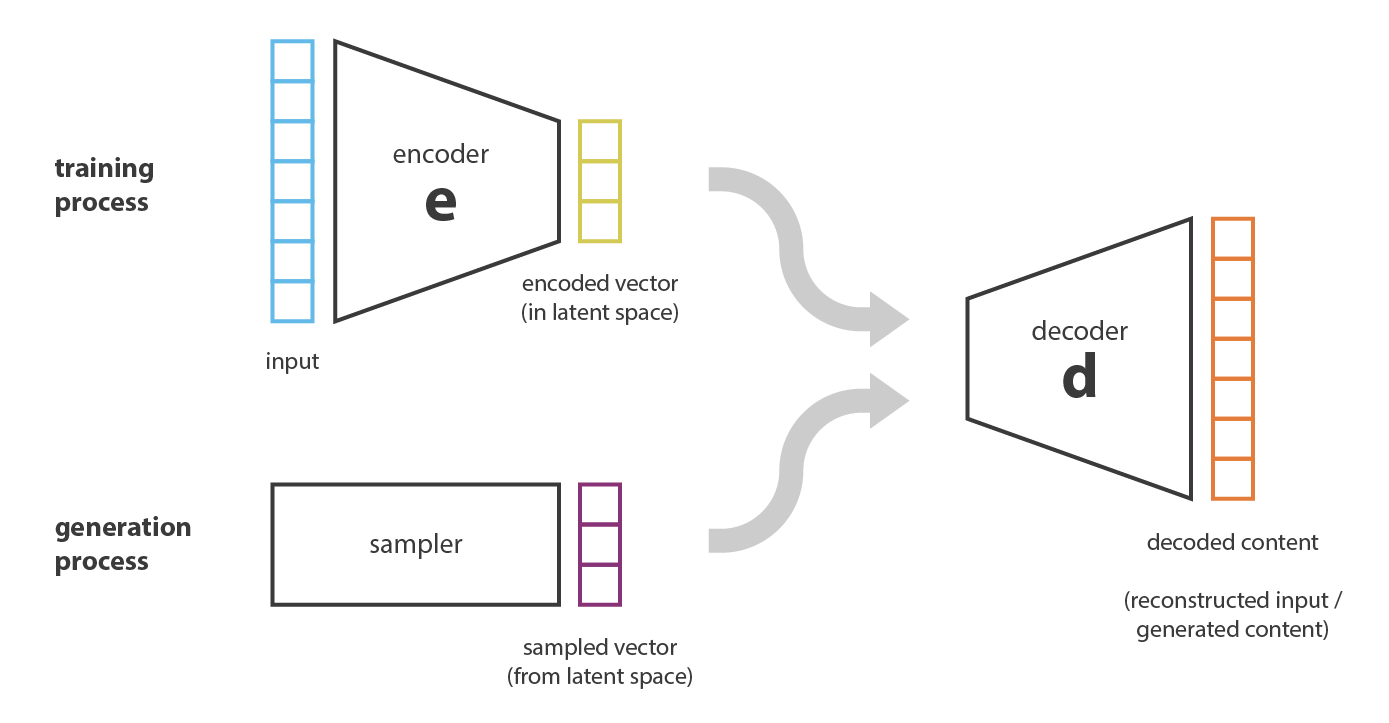
\includegraphics[width= \linewidth]{VAE.png}
    \caption{\label{fig: VAE} Diagram of Variational Autoencoder from \cite{rocca_2020}}
  }
\end{figure}

An interesting spin on this concept is that of Variational Autoencoders (VAEs). In addition to being able to reconstruct inputs, VAEs treat the latent code $z$ as a random variable distributed according to some prior distribution $p(z)$. This then gives new interpretations to both the encoder and decoder portions of the network. The encoder of the inputs $x$ can be thought as an approximator $q(z | x)$ of the posterior of this distribution $p(z | x)$ and the decoder gives an approximation of the distribution over the inputs conditional to a given value of $z$ (i.e. $p(x | z)$). Generating new samples with this framework then consists of $z \sim p(z)$ and $x \sim p(x | z)$.

Training VAEs then becomes a problem of optimizing an objective of the form 

\[
  \mathcal{L}_1(x; \theta, \phi) = E[\log ~ p_\theta (x | z)] - KL(q_\phi(z | x) || p(z))
\]

where $\theta$ and $\phi$ represent the parameters of the decoder and encoder portions of the VAE respectively and $KL(\cdot || \cdot)$ is the Kullback-Leibler divergence.

Following the example of (Roberts et al., 2018), we follow a slightly different objective 

\begin{align*}
  & \mathcal{L}_2(x; \theta, \phi, \tau, \beta) = \\
   & E[\log ~ p_\theta (x | z)] - \beta \max(KL(q_\phi(z | x) || p(z)) - \tau, 0)
\end{align*}

which follows from the interpretation that the KL-divergence measures the amount of information required to code samples from $p(z)$ using $q_\phi(z | x)$. $\tau$ then parametrizes a ``free information budget'' to be used while learning to approximate the posterior and $\beta$ allows to trade off between accurate reconstructions and learning a compact latent code.

\section{Models}
\subsection{Simple Approach}
 The first utilized architecture is composed of 3 stacked LSTM layers with 64 units each using tanh activation between each layer. A fully connected layer with softmax activation was used for the output. The final configuration for this network was found using a box-search over the number of layers and number of units in each layer.

\subsection{Hierarchical Decoder VAE Approach}

One of the prominent problems when using generative latent variable models such as VAE to generate sequences is that of the ``posterior collapse''. The problem arises when the variational distribution of latent variables closely matches that of the uninformative prior (Lucas et al., 2019)\cite{lucas2019understanding}. In other words, the output of the sequence learns to generate outputs according to some overall distribution $p(z)$, but fails to utilize other information available. When generating musical tracks, this often manifests as repetitive sequences that lack long term structure.

The architecture in (Roberts et al., 2018) shown in \textbf{Figure ~\ref{fig:hierarchical}} attempts to mitigate this by having all portions of the generated sequence depend closely on the latent code.

\begin{figure}[H]
  \center{
    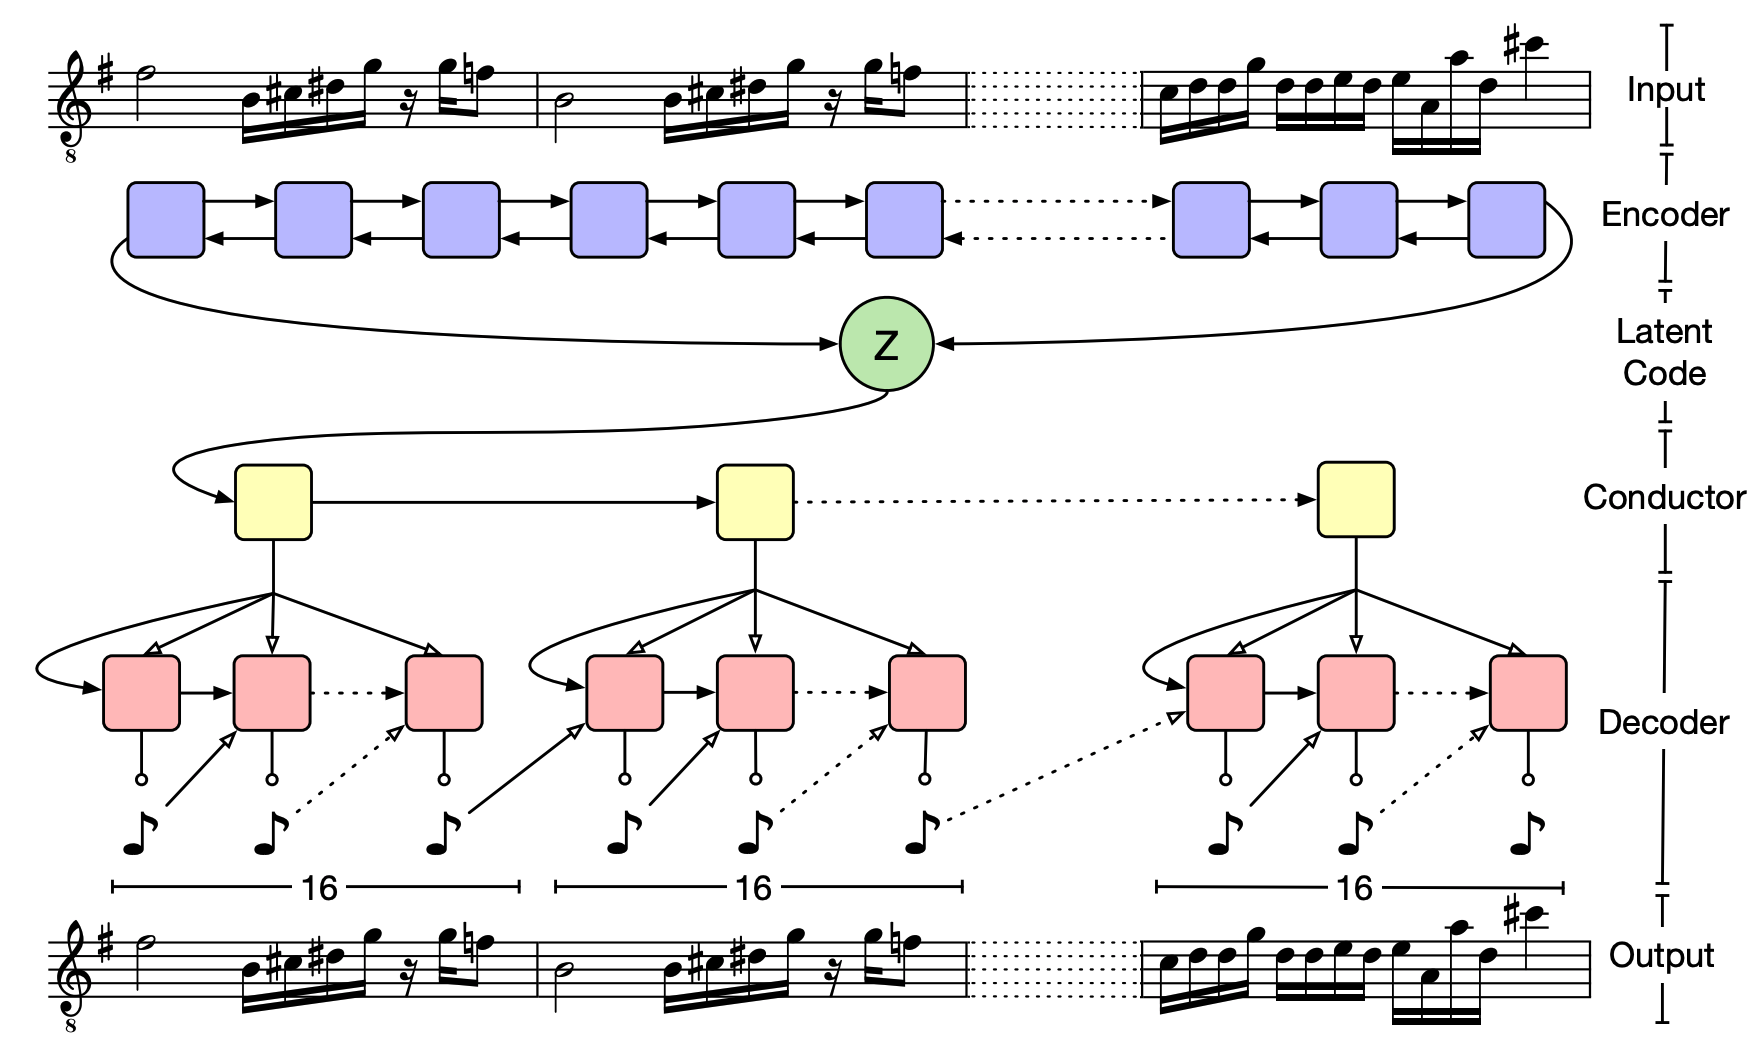
\includegraphics[width=\linewidth]{hierarchical.png}
    \caption{\label{fig:hierarchical} Hierarchical Decoder VAE from \cite{roberts2018hierarchical}}
  }
\end{figure}

\subsubsection{Encoder Portion}
This architecture first uses a 2-layer bidirectional LSTM to process a sequence of inputs $x = \{ x_1, x_2, \hdots, x_T \}$ and utilizes the concatenation of the last hidden state vectors of the second layer $\overrightarrow{h_T}$ and $\overleftarrow{h_T}$ as the input to a fully connected layer that is used to calculate the distributional parameters of the latent code of the VAE according to 

\begin{align*}
  \mu &= W_{h\mu} h_T + b_\mu \\
  \sigma &= \log(\exp(W_{h\sigma} h_T + b_\sigma) + 1)
\end{align*}

Where $W_h\mu$, $h_T$, $b_\mu$, and $b_\sigma$ are weight matrices and bias vectors respectively. Following the architecture design described in (Roberts et al., 2018), all hidden states have size 2048 and the latent code has size 512. The latent vector $z$ is then drawn from a multivariate gaussian distribution with mean $\mu$ and covariance matrix equal to a diagonal matrix with the entries of $\sigma$ along its diagonal.

\subsubsection{Decoder Portion}
The decoding of $z$ is then a two-step approach that first generates embedding vectors $c = \{ c_1, c_2, ..., c_U \}$, one for each of the $U$ subsequence to be generated, by passing $z$ as the initial state to the so-called conductor RNN. Each of those embeddings is then decoded independently by a separate RNN to produce the $U$ output sequences which in turn get concatenated to produce the final result. In order to encourage dependance on the latent code, the input of the RNN was constantly augmented with the corresponding embedding vector at each decoding step.

For the experiments, both the conductor and decoder networks are implemented using two-layer unidirectional LSTMs with hidden size of 1024 and output dimension of 512. In the decoding step, softmax activation was used and the 512 output units corresponds to all the possible combinations of the 9 percussion instruments considered ($2^9 = 512$).

\section{Experiments}

\subsection{Data Processing and Training}
All the drum tracks utilized throughout the experiments came from the public Lakh MIDI data-set (Raffel et al., 2019)\cite{raffel2016extracting} which contains a variety of 176,581 unique MIDI files. Using MIDI files as a data source is convenient because they store music as a sequence of messages that specify which instruments are playing at any given time. During processing, each bar is divided into 16 equal regions and message values are averaged to obtain the value of that region. To reduce the complexity of the model, rather than using the 61 different percussion classes specified by the General MIDI standard, instruments were mapped into the 9 canonical classes. At each step, the state of the instruments was then encoded using a one-hot representation with 512 possible values; one for each of the possible combinations of the 9 instruments.

To see the relation in the performance of the different models and the length of the sequences produced, two sequence lengths are considered. The short sequences are composed 2-bar drum patterns and long sequences of 16-bar drum patterns. To extract sequences of the appropriate size, we iterate over the available samples using only the percussion channel with a window of the desired size and output all sequences that match the window size. For the hierarchical approach, subsequences have size 16 and therefore correspond to a bar in the track.

Following the specifications on (Roberts et al., 2018), all models are trained with Adam with a learning rate that goes from $10^{-3}$ to $10^{-5}$ with an exponential decay rate of $0.9999$ and batch size of 512.

\subsection{Reconstruction Quality}
To test the ability of the different models to learn the given musical sequences, we compare their ability to reconstruct the original input sequences. For each configuration, two training approaches were explored: teacher-forcing and scheduled sampling.

During teacher-forcing, the model is given the ground truth from previous time-steps. Having access to the ground truth helps the model converge faster as it does not have to learn over compounding errors. This however, creates a discrepancy between training and generating sequences where the ground truth is not available. As a middle ground, we also experiment with scheduled sampling where we choose whether to feed in the ground truth or the predicted output of previous steps based on some Bernoulli random variable with probability $p$. For our experiments, we used $p = 0.5$.

\subsubsection{Simple Approach}

\begin{table}[H]
\setlength{\tabcolsep}{3pt}
\centering
\begin{tabular}{@{} l SSSSS @{}} % @{} serves to suppress white space at ends of table
\toprule
Sequence & {Teacher-Forcing} & {Sampling} \\
\midrule
2-bar Drum & 0.969 & 0.931 \\
16-bar Drum & 0.634 & 0.459 \\
\bottomrule
\end{tabular}
\caption{\label{tab:reconstruct_simple} Reconstruction Accuracies}
\end{table}
For 2-bar sequences (length = 32), reconstructions based on our simple architecture produced great results. For the most part, both learning approaches only differed from the actual inputs on one or two time-steps. Despite this success, this model was not able to reliable reconstruct 16-bar sequences as shown by the reconstruction accuracies on \textbf{table \ref{tab:reconstruct_simple}}. After carefully examining the generated outputs, it is evident that the model regressed to constantly predicting the most frequently occurring note in the input. An example of this phenomenon is shown in \textbf{figure \ref{fig:example-seq}}.

\begin{figure}[H]
  \begin{subfigure}{0.5\textwidth}
    \centering
    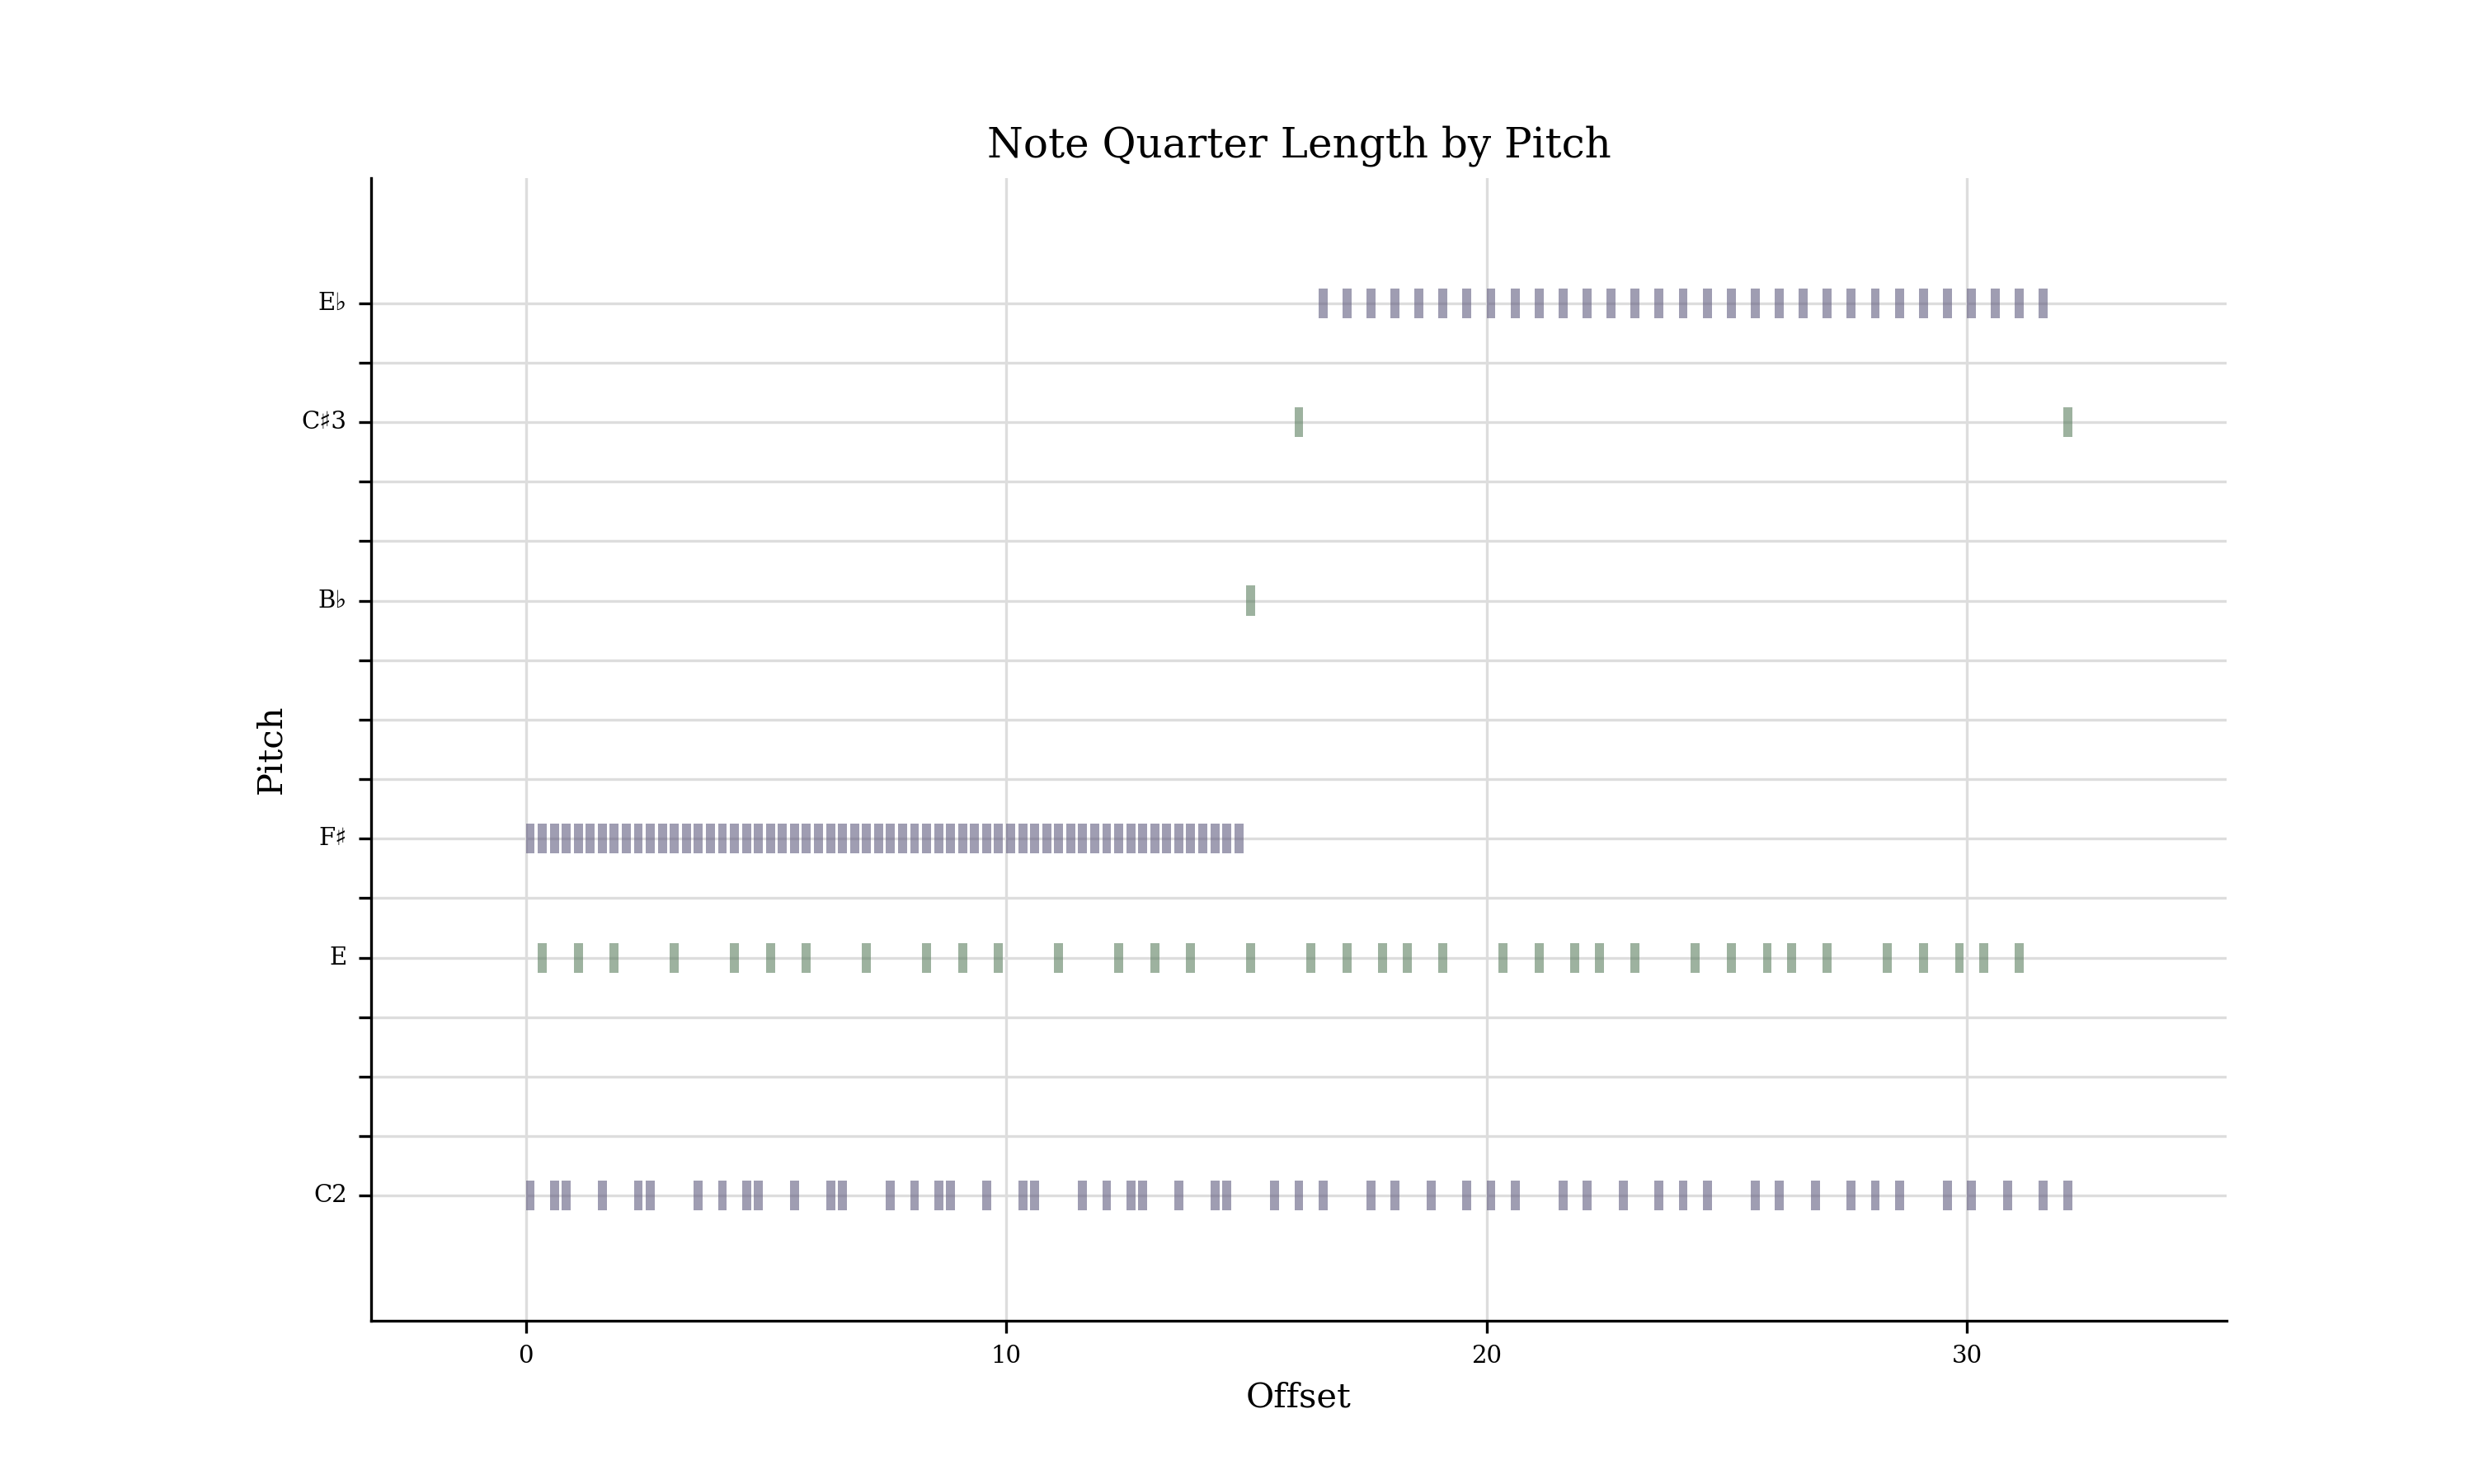
\includegraphics[width=0.9 \linewidth]{actual.png}
    \caption{Input Sequence}
  \end{subfigure}

  \begin{subfigure}{0.5\textwidth}
    \centering
    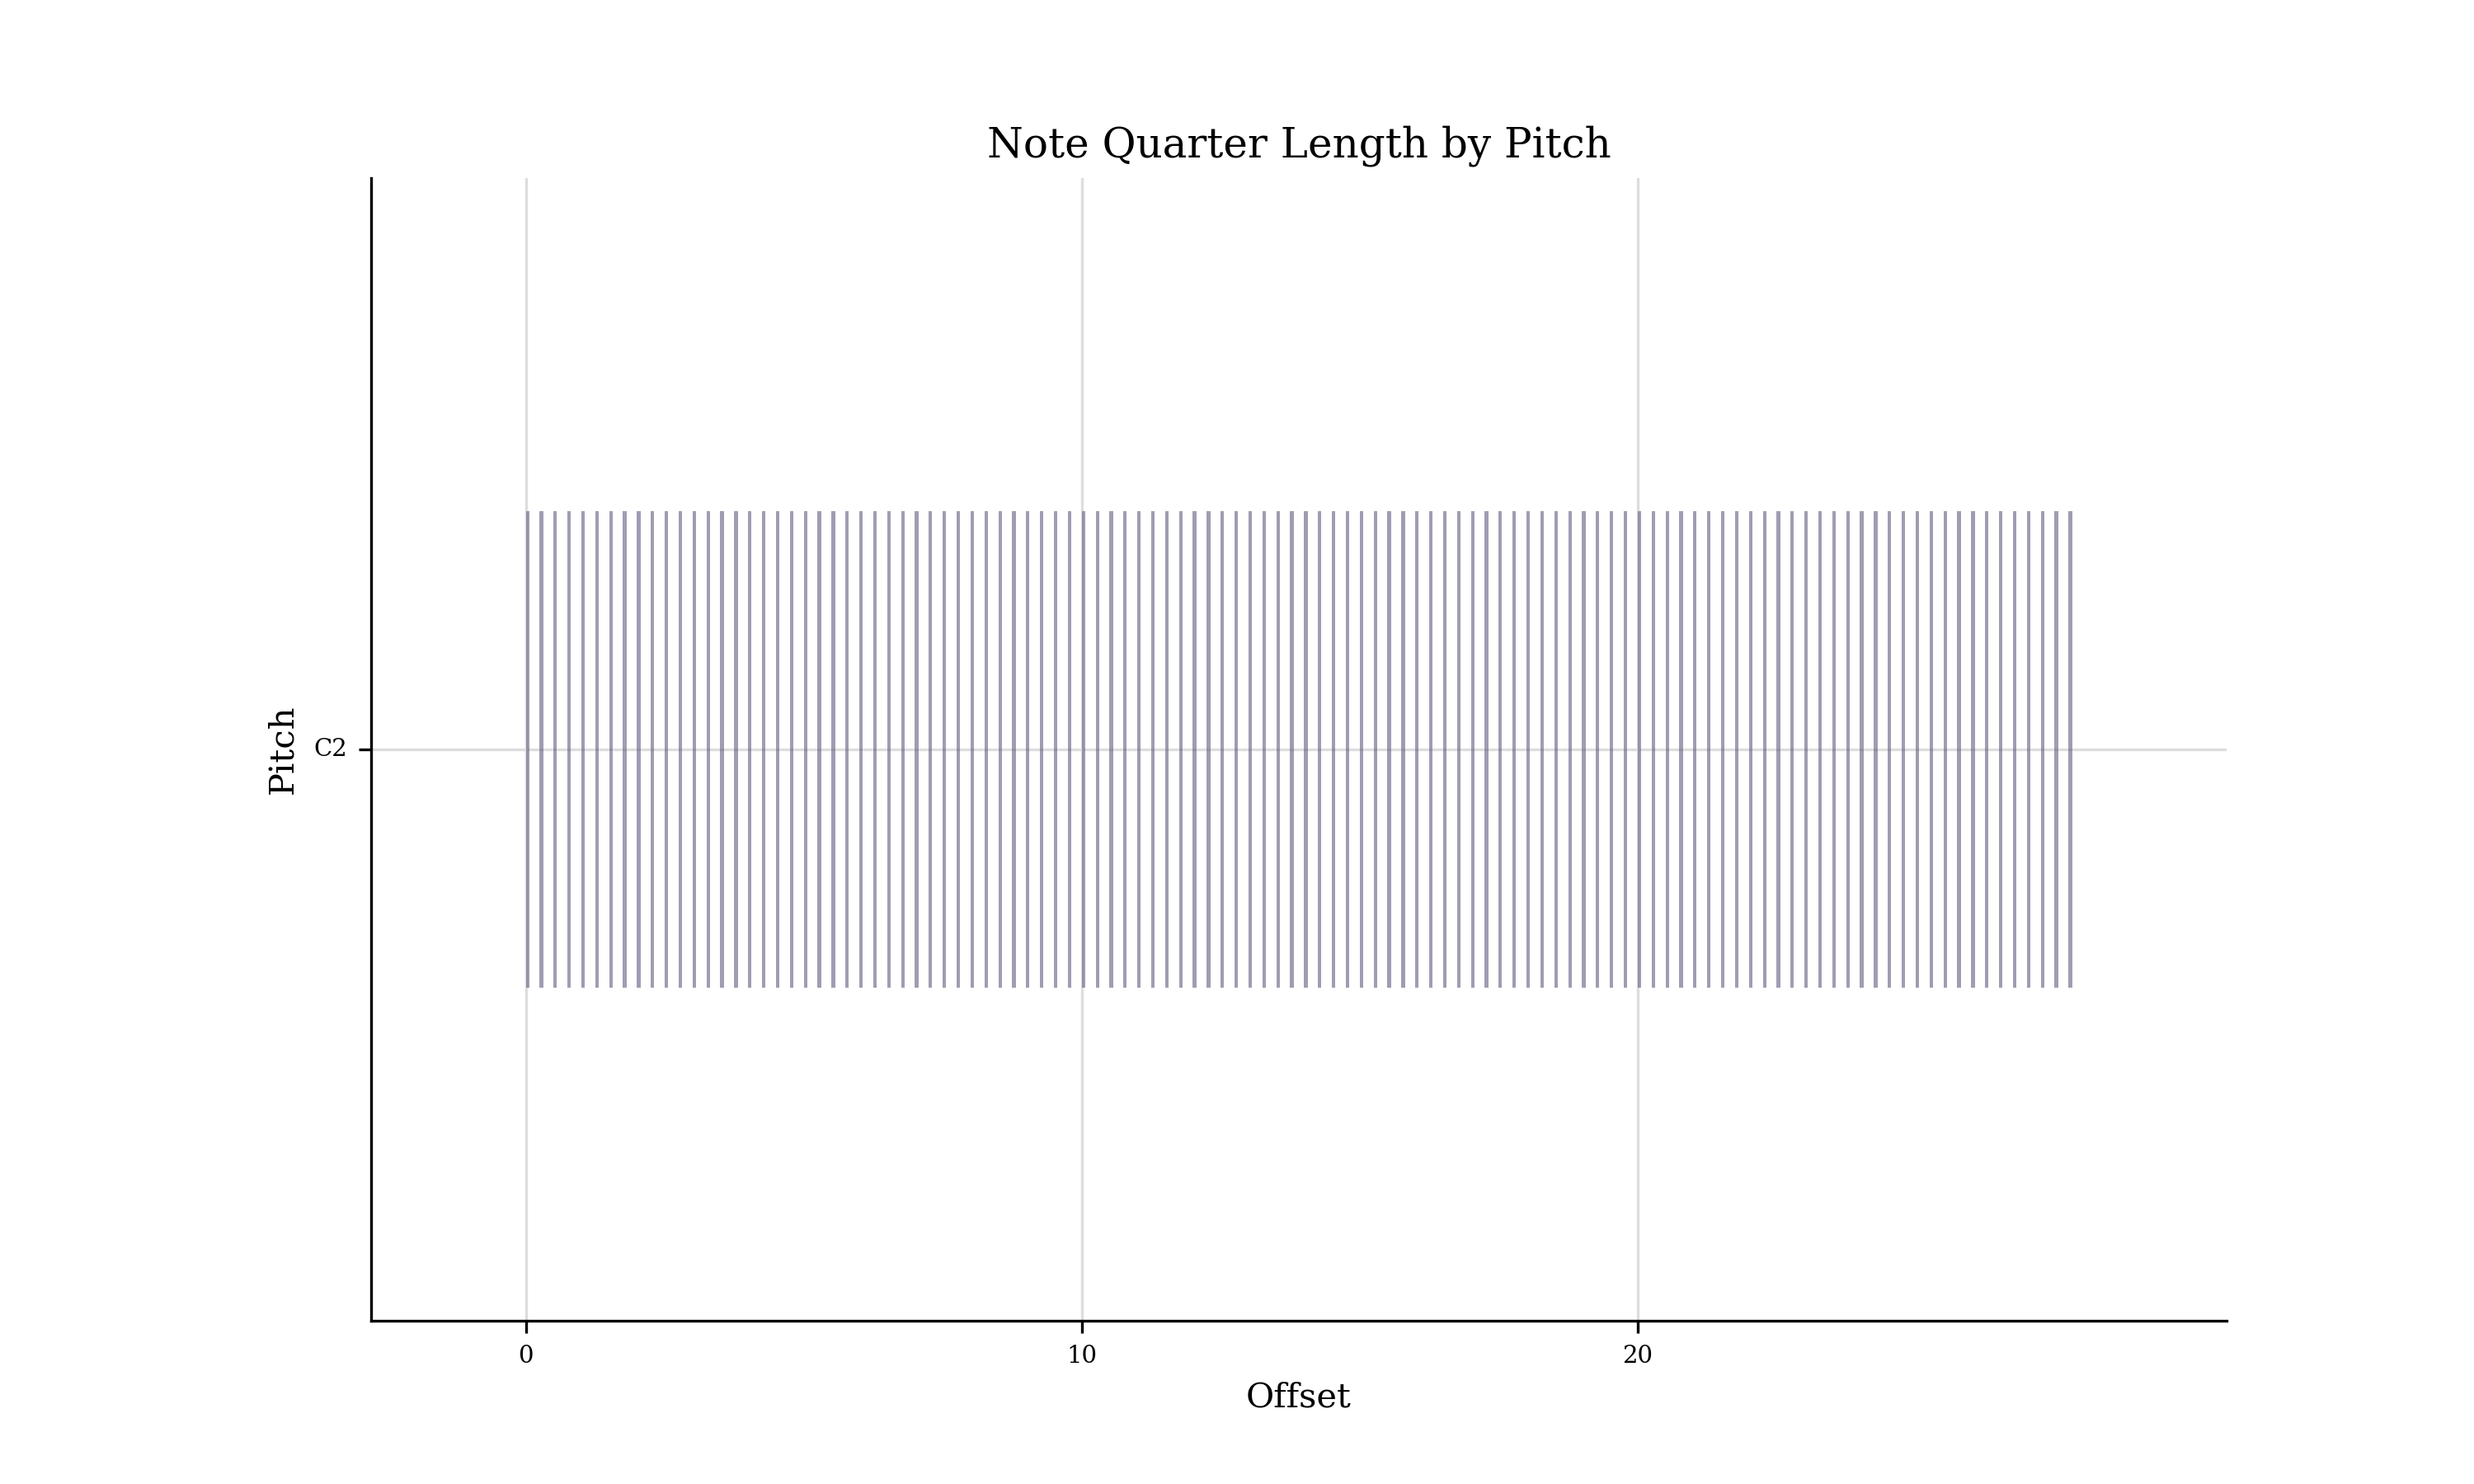
\includegraphics[width=0.9 \linewidth]{predicted.png}
    \caption{Predicted Sequence}
  \end{subfigure}
  \caption{Example of 16-bar Output Sequence}
  \label{fig:example-seq}
\end{figure}

\subsubsection{Recurrent Variational Autoencoders}
\begin{table}[H]
\setlength{\tabcolsep}{3pt}
\centering
\begin{tabular}{@{} l SSSSS @{}} % @{} serves to suppress white space at ends of table
\toprule
Model &  \multicolumn{2}{c @{}}{Teacher-Forcing} & \multicolumn{2}{c @{}}{Sampling} \\ 

\cmidrule(l){2-5}
    & {Flat} & {Hierarchical} & {Flat} & {Hierarchical} \\
\midrule
2-bar Drum & 0.982 & 0.963 & 0.905 & 0.924 \\
16-bar Drum & 0.852 & 0.943 & 0.621 & 0.893 \\
\bottomrule
\end{tabular}
\caption{\label{tab:reconstruct_vae} Reconstruction Accuracies}
\end{table}

For the 2-bar sequences, both the flat decoder and hierarchical decoder architectures did quite well and were able to reconstruct the sequences almost perfectly. In most cases, predictions only had one or two discrepancies and were audibly indistinguishable from the real inputs. This was to be expected because the task was basically to recreate a repetitive sequence of length 32 with mostly no drastic changes in structure. However, when analyzing the results wile attempting to do the same task on 16-bar sequences, the performance of the models was significantly different. When looking at the accuracy differences obtained using the teacher-forcing and scheduled sampling methods, the flat architecture showed a substantially larger performance drop (23.1\%) where the hierarchical architecture only lost a 5.0\% drop in accuracy. If we consider that longer sequences tend to have more variations on the repetitive structure of the drum pattern, this can be interpreted as evidence of the superior ability of the hierarchical architecture to learn the concept of a long-term structure in a drum piece.

\subsection{Track Generation and Listening Tests}
For the lack of a better quantitative way to measure the quality of generated samples using the VAE architectures, 32 people were polled and asked to do pair-wise comparisons of track pairs. To create each pair, we first selected 10 random samples from both the flat and hierarchical VAE architectures as well as 10 samples from the original data-set and then randomly sample one element from the two groups to be compared. Each person was presented with 42 pairwise comparisons that were evenly split between the possible category pairings and were asked to identify which track they believed to be ``more musical''. The number of times that each category was selected as the more musical one is depicted in \textbf{figure \ref{fig:num_wins}}.

\begin{figure}[H]
  \center{
    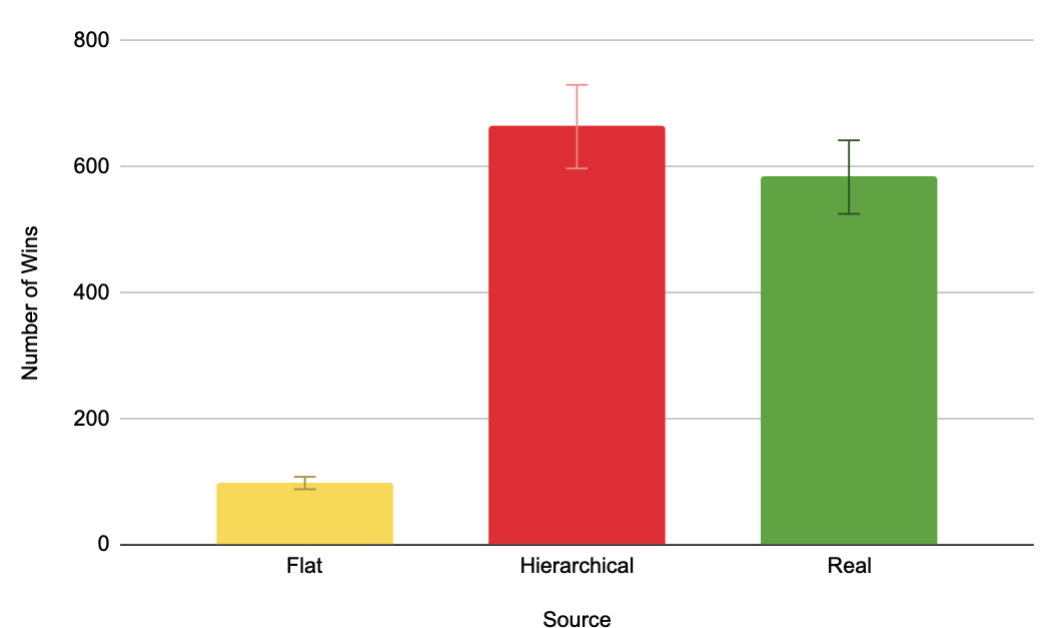
\includegraphics[width=\linewidth]{Comparisons.png}
  }
  \caption{Number of wins per category}
  \label{fig:num_wins}
\end{figure}

As depicted in figure \ref{fig:num_wins} the hierarchical architecture was chosen at a much higher rate that flat version and at a slightly higher rate than that of the real samples. The difference in rate at which real samples and samples generated using the hierarchical architecture, however, was not statistically significant.

\section{Conclusion}

We explored two different methods to generate percussive sound tracks; one that treats music generation as a time-series prediction problem and the other that uses a VAE with a decoder with a hierarchical architecture. Empirically, we found that both the simple approach and the VAE approach with a flat recurrent decoder were prone to the posterior collapse problem and tend to fail to capture the long term structure of longer sequences. As such, their outputs tend to be very repetitive and unpleasantly sounding. Additionally, we verified that the quality of generated outputs using the hierarchical VAE was comparable to that of the original samples.

% Page Break before references %
\pagebreak

\bibliographystyle{abbrv}
\bibliography{refs}
\end{document}
